\documentclass{beamer}
% =============================================================================
% ENCODING
% =============================================================================
\usepackage[utf8]{inputenc}  % UTF-8 encoding support

% =============================================================================
% GRAPHICS
% =============================================================================
\usepackage{graphicx}  % For \includegraphics (401 uses across lectures)

% =============================================================================
% MATH PACKAGES
% =============================================================================
\usepackage{amsmath}    % For align, multline, equation environments (heavily used)
\usepackage{amsfonts}   % For \mathbb (e.g., \bbR, \bbE)
\usepackage{amssymb}    % For additional math symbols

% =============================================================================
% TABLES
% =============================================================================
\usepackage{booktabs}   % For \toprule, \midrule, \bottomrule (used in lecture13, lecture14)

% =============================================================================
% LISTS
% =============================================================================
\usepackage{enumerate}  % Enhanced enumerate environment (76 uses across lectures)

% =============================================================================
% TIKZ (DIAGRAMS)
% =============================================================================
\usepackage{tikz}       % For taxonomy diagram and footnotes positioning

% =============================================================================
% UTILITY PACKAGES
% =============================================================================
\usepackage{multido}    % For \multido command used in \eqpause
\usepackage{etoolbox}   % For \AtEndEnvironment, \ifbool, \newbool (used in preamble and taxonomy)
\usepackage{xspace}     % For smart spacing after custom commands (\ODESolve, \SDESolve)

% =============================================================================
% BEAMER THEME SETTINGS
% =============================================================================
\usetheme{default}
\usecolortheme{default}

\setbeamerfont{title}{size=\Huge}
\setbeamertemplate{footline}[frame number]{}
\setbeamertemplate{section in toc}[sections numbered]

\makeatletter
\newcommand\HUGE{\@setfontsize\Huge{35}{40}}
\makeatother    

\setbeamerfont{title}{size=\HUGE}
\beamertemplatenavigationsymbolsempty

% =============================================================================
% TIKZ LIBRARIES
% =============================================================================
% Used for taxonomy diagram: arrows, positioning, shapes
\usetikzlibrary{arrows.meta,calc,shapes,positioning,shadows,trees}

% =============================================================================
% CUSTOM FOOTNOTE COMMANDS
% =============================================================================
% \myfootnote{text} - creates a footnote at the bottom of the slide
\newcommand\myfootnote[1]{%
  \vspace{-0.5cm}%
  \tikz[remember picture,overlay]
  \draw (current page.south west) +(1in + \oddsidemargin,0.5em)
  node[anchor=south west,inner sep=0pt]{\parbox{\textwidth}{%
      \rlap{\rule{10em}{0.4pt}}\raggedright\scriptsize \textit{#1}}};}

% \myfootnotewithlink{url}{text} - creates a clickable footnote (623 uses across lectures)
\newcommand\myfootnotewithlink[2]{%
  \vspace{-0.5cm}%
  \tikz[remember picture,overlay]
  \draw (current page.south west) +(1in + \oddsidemargin,0.5em)
  node[anchor=south west,inner sep=0pt]{\parbox{\textwidth}{%
      \rlap{\rule{10em}{0.4pt}}\raggedright\scriptsize\href{#1}{\textit{#2}}}};}

% =============================================================================
% SECTION/SUBSECTION OUTLINE AUTOMATION
% =============================================================================
% Automatically show outline at the beginning of each section
\AtBeginSection[]
      {
      	\begin{frame}{Outline}
      		\tableofcontents[currentsection]
      	\end{frame}
      }
      \AtBeginSubsection[]{
      	\begin{frame}{Outline}
      		\tableofcontents[currentsection,currentsubsection]
      	\end{frame}
}

% =============================================================================
% CUSTOM SLIDE ANIMATION COMMANDS
% =============================================================================
% These commands enable step-by-step reveal of equations and content
% Used heavily across all lectures (1130+ uses of \nextonslide and \eqpause)

\newcounter{noscounter}   % Counter for \nextonslide (resets on each new slide)
\newcounter{pcounter}     % Counter for pause commands (resets after \eqpause)
\newcounter{diffcounter}  % Counts pauses after equations

% \nextonslide{content} - reveals content on the next overlay
\newcommand{\nextonslide}[1]{%
  \stepcounter{noscounter}%
  \stepcounter{pcounter}%
  \stepcounter{diffcounter}%
  \onslide<\value{noscounter}->{#1}%
}

% \resetonslide - resets all animation counters (called at each frame)
\newcommand{\resetonslide}{%
    \setcounter{noscounter}{1}%
    \setcounter{pcounter}{1}%
    \setcounter{diffcounter}{0}%
}

% \eqpause - pause after equation that syncs with \nextonslide
\newcommand{\eqpause}{%
  \multido{\i=1+1}{\value{pcounter}}{\pause}%
  \stepcounter{noscounter}%
  \setcounter{pcounter}{1}%
}

% \eqpausediff - helper command, runs automatically after math environments
\newcommand{\eqpausediff}{%
  \multido{\i=1+1}{\value{diffcounter}}{\pause}%
  \addtocounter{pcounter}{-\value{diffcounter}}%
  \setcounter{diffcounter}{0}%
}

% Apply \eqpausediff after math environments
\newcommand\AtEndBoth[2]{%
  \AtEndEnvironment{#1}{#2}%
  \AtEndEnvironment{#1*}{#2}%
}

\AtEndBoth{align}{\eqpausediff}
\AtEndBoth{equation}{\eqpausediff}
\AtEndBoth{multline}{\eqpausediff}

% Reset counters at the beginning of each frame
\addtobeamertemplate{frametitle}{\resetonslide}{}

% =============================================================================
% INCLUDE OTHER CONFIGURATION FILES
% =============================================================================
% ==============================================================================
% Custom LaTeX Commands for Deep Generative Models Course
% ==============================================================================

% ==============================================================================
% BOLD LETTERS (mathbf / boldsymbol)
% ==============================================================================

% ------------------------------------------------------------------------------
% Latin Bold Lowercase
% Usage: \bx for x in bold, commonly used for vectors
% ------------------------------------------------------------------------------
\newcommand{\ba}{\mathbf{a}}
\newcommand{\bc}{\mathbf{c}}
\newcommand{\be}{\mathbf{e}}
\newcommand{\bff}{\mathbf{f}}  % Note: \bf is reserved for bold font switching
\newcommand{\bg}{\mathbf{g}}
\newcommand{\bh}{\mathbf{h}}
\newcommand{\bp}{\mathbf{p}}
\newcommand{\bq}{\mathbf{q}}
\newcommand{\bs}{\mathbf{s}}
\newcommand{\bt}{\mathbf{t}}
\newcommand{\bu}{\mathbf{u}}
\newcommand{\bv}{\mathbf{v}}
\newcommand{\bw}{\mathbf{w}}
\newcommand{\bx}{\mathbf{x}}
\newcommand{\by}{\mathbf{y}}
\newcommand{\bz}{\mathbf{z}}
\newcommand{\bzero}{\boldsymbol{0}}  % Zero vector
\newcommand{\bone}{\mathbf{1}}       % Ones vector

% ------------------------------------------------------------------------------
% Latin Bold Uppercase
% Usage: \bX for X in bold, commonly used for matrices or random vectors
% ------------------------------------------------------------------------------
\newcommand{\bA}{\mathbf{A}}
\newcommand{\bG}{\mathbf{G}}
\newcommand{\bI}{\mathbf{I}}
\newcommand{\bJ}{\mathbf{J}}
\newcommand{\bL}{\mathbf{L}}
\newcommand{\bM}{\mathbf{M}}
\newcommand{\bP}{\mathbf{P}}
\newcommand{\bQ}{\mathbf{Q}}
\newcommand{\bR}{\mathbf{R}}
\newcommand{\bT}{\mathbf{T}}
\newcommand{\bU}{\mathbf{U}}
\newcommand{\bV}{\mathbf{V}}
\newcommand{\bW}{\mathbf{W}}
\newcommand{\bX}{\mathbf{X}}
\newcommand{\bZ}{\mathbf{Z}}

% ------------------------------------------------------------------------------
% Greek Bold Lowercase
% Usage: \btheta for θ in bold, commonly used for parameter vectors
% ------------------------------------------------------------------------------
\newcommand{\bepsilon}{\boldsymbol{\epsilon}}
\newcommand{\blambda}{\boldsymbol{\lambda}}
\newcommand{\bmu}{\boldsymbol{\mu}}
\newcommand{\bphi}{\boldsymbol{\phi}}
\newcommand{\bpi}{\boldsymbol{\pi}}
\newcommand{\bpsi}{\boldsymbol{\psi}}
\newcommand{\bsigma}{\boldsymbol{\sigma}}
\newcommand{\btheta}{\boldsymbol{\theta}}

% ------------------------------------------------------------------------------
% Greek Bold Uppercase
% Usage: \bSigma for Σ in bold, commonly used for covariance matrices
% ------------------------------------------------------------------------------
\newcommand{\bPhi}{\boldsymbol{\Phi}}
\newcommand{\bSigma}{\boldsymbol{\Sigma}}
\newcommand{\bTheta}{\boldsymbol{\Theta}}

% ==============================================================================
% CALLIGRAPHIC LETTERS (mathcal)
% Usage: \cX for calligraphic X, commonly used for sets and spaces
% ==============================================================================
\newcommand{\cF}{\mathcal{F}}
\newcommand{\cI}{\mathcal{I}}
\newcommand{\cL}{\mathcal{L}}
\newcommand{\cM}{\mathcal{M}}
\newcommand{\cN}{\mathcal{N}}
\newcommand{\cO}{\mathcal{O}}
\newcommand{\cP}{\mathcal{P}}
\newcommand{\cS}{\mathcal{S}}
\newcommand{\cT}{\mathcal{T}}
\newcommand{\cW}{\mathcal{W}}
\newcommand{\cX}{\mathcal{X}}
\newcommand{\cZ}{\mathcal{Z}}

% ==============================================================================
% BLACKBOARD BOLD LETTERS (mathbb)
% Usage: \bbR for ℝ, commonly used for number sets and expectations
% ==============================================================================
\newcommand{\bbE}{\mathbb{E}}  % Expectation
\newcommand{\bbI}{\mathbb{I}}  % Indicator function
\newcommand{\bbP}{\mathbb{P}}  % Probability measure
\newcommand{\bbR}{\mathbb{R}}  % Real numbers

% ==============================================================================
% MATH OPERATORS
% ==============================================================================

% ------------------------------------------------------------------------------
% Optimization Operators
% Usage: \argmin_{x} f(x) for proper spacing and limits placement
% ------------------------------------------------------------------------------
\DeclareMathOperator*{\argmin}{arg\,min}
\DeclareMathOperator*{\argmax}{arg\,max}

% ------------------------------------------------------------------------------
% Statistical Operators
% Usage: \cov(X, Y) for covariance
% ------------------------------------------------------------------------------
\DeclareMathOperator{\cov}{cov}

% ------------------------------------------------------------------------------
% Linear Algebra Operators
% Usage: \tr(\bA) for trace of matrix A
% ------------------------------------------------------------------------------
\DeclareMathOperator{\tr}{tr}

% ------------------------------------------------------------------------------
% Other Mathematical Operators
% ------------------------------------------------------------------------------
\DeclareMathOperator{\diver}{div}      % Divergence (vector calculus)
\newcommand{\sg}{\mathrm{sg}}          % Stop-gradient operator
\DeclareMathOperator{\softmax}{softmax}
\DeclareMathOperator{\supp}{supp}      % Support of a distribution

% ==============================================================================
% PROBABILITY DISTRIBUTIONS
% Usage: X \sim \cN(0, 1), Y \sim \Bern(p)
% ==============================================================================
\DeclareMathOperator{\Bern}{Bern}      % Bernoulli distribution
\DeclareMathOperator{\Cat}{Cat}        % Categorical distribution
\DeclareMathOperator{\Gumbel}{Gumbel}  % Gumbel distribution
\DeclareMathOperator{\Uniform}{Uniform}

% ==============================================================================
% METRICS AND DIVERGENCES
% Usage: \KL(p \| q), \JSD(p, q)
% ==============================================================================
\newcommand{\Ent}{\mathrm{H}}          % Entropy
\newcommand{\FID}{\mathrm{FID}}        % Fréchet Inception Distance
\newcommand{\JSD}{D_\mathrm{JS}}        % Jensen-Shannon Divergence
\newcommand{\KL}{D_\mathrm{KL}}        % Kullback-Leibler Divergence
\DeclareMathOperator{\MMD}{MMD}        % Maximum Mean Discrepancy
\DeclareMathOperator{\SNR}{SNR}        % Signal-to-Noise Ratio

% ==============================================================================
% NEURAL NETWORK NOTATION
% ==============================================================================

% ------------------------------------------------------------------------------
% Network Architectures (upright font for abbreviations)
% Usage: f_{\btheta} = \NN_{\btheta}(\bx)
% ------------------------------------------------------------------------------
\newcommand{\MLP}{\mathrm{MLP}}        % Multi-Layer Perceptron
\newcommand{\NN}{\mathrm{NN}}          % Neural Network
\newcommand{\RNN}{\mathrm{RNN}}        % Recurrent Neural Network

% ------------------------------------------------------------------------------
% Numerical Solvers (monospace font)
% Usage: \bx_T = \ODESolve(v, \bx_0, T)
% ------------------------------------------------------------------------------
\newcommand{\ODESolve}{\texttt{ODESolve}\xspace}
\newcommand{\SDESolve}{\texttt{SDESolve}\xspace}

% ==============================================================================
% COMMON SHORTCUTS
% Usage: Frequently used subscripted or parameterized expressions
% ==============================================================================
\newcommand{\pd}{p_{\text{data}}}              % Data distribution
\newcommand{\pt}{p_{\boldsymbol{\theta}}}      % Parameterized distribution
\newcommand{\qagg}{q_{\text{agg}}}             % Aggregated posterior
\newcommand{\lambdamax}{\lambda_{\text{max}}}  % Maximum eigenvalue
  % Math shorthand commands (\bx, \bbE, \KL, etc.)
\input{../utils/title}        % Title page template
% For each possible node, we create a boolean
\newbool{hl@root}
\newbool{hl@explicit}
\newbool{hl@implicit}
\newbool{hl@exact}
\newbool{hl@approx}
\newbool{hl@gan}
\newbool{hl@ar}
\newbool{hl@nf}
\newbool{hl@vae}
\newbool{hl@score}
\newbool{hl@cont}
\newbool{hl@ddpm}
\newbool{hl@sm}
\newbool{hl@ode}
\newbool{hl@sde}
\newbool{hl@fm}

% Command to reset all bools
\newcommand{\resetAllHighlights}{%
    \boolfalse{hl@root}%
    \boolfalse{hl@explicit}%
    \boolfalse{hl@implicit}%
    \boolfalse{hl@exact}%
    \boolfalse{hl@approx}%
    \boolfalse{hl@gan}%
    \boolfalse{hl@ar}%
    \boolfalse{hl@nf}%
    \boolfalse{hl@vae}%
    \boolfalse{hl@score}%
    \boolfalse{hl@cont}%
    \boolfalse{hl@ddpm}%
    \boolfalse{hl@sm}%
    \boolfalse{hl@ode}%
    \boolfalse{hl@sde}%
    \boolfalse{hl@fm}%
}

% Command to set a single highlight
\newcommand{\setHighlight}[1]{%
    \booltrue{hl@#1}%
}

% Command to set highlights from comma-separated list
\newcommand{\setHighlights}[1]{%
    \resetAllHighlights%
    \forcsvlist{\setHighlight}{#1}%
}

% Highlighted style definition
\tikzset{
    hl/.style={line width=1.2pt, draw=black, font=\scriptsize\bfseries},
    box/.style={
        rectangle, 
        draw=gray!50, 
        rounded corners=2pt, 
        minimum width=1.9cm, 
        minimum height=0.5cm, 
        align=center, 
        font=\scriptsize, 
        line width=0.4pt
    },
    rootnode/.style={box, fill=violet!20},
    category/.style={box, fill=teal!20},
    model/.style={box, fill=yellow!30},
    arrow/.style={-Stealth, draw=gray!80, line width=0.4pt}
}

% Draw taxonomy with pre-set highlights
\newcommand{\drawTaxonomy}{%
    \begin{tikzpicture}[scale=0.9, transform shape, node distance=0.6cm and 0.3cm]
        % --- CENTRAL ROOT ---
        \ifbool{hl@root}{\node[rootnode, hl] (root) {Generative Models};}{\node[rootnode] (root) {Generative Models};}

        % --- UPPER BRANCHES ---
        \ifbool{hl@explicit}{\node[category, hl, above left=0.6cm and 0.5cm of root] (explicit) {Explicit density};}{\node[category, above left=0.6cm and 0.5cm of root] (explicit) {Explicit density};}
        \ifbool{hl@implicit}{\node[category, hl, above right=0.6cm and 0.5cm of root] (implicit) {Implicit density};}{\node[category, above right=0.6cm and 0.5cm of root] (implicit) {Implicit density};}

        \ifbool{hl@exact}{\node[category, hl, above left=0.6cm and -0.6cm of explicit] (exact) {Exact likelihood};}{\node[category, above left=0.6cm and -0.6cm of explicit] (exact) {Exact likelihood};}
        \ifbool{hl@approx}{\node[category, hl, above right=0.6cm and -0.6cm of explicit] (approx) {Approximate likelihood};}{\node[category, above right=0.6cm and -0.6cm of explicit] (approx) {Approximate likelihood};}

        \ifbool{hl@gan}{\node[model, hl, above=0.6cm of implicit] (gans) {GANs};}{\node[model, above=0.6cm of implicit] (gans) {GANs};}

        \ifbool{hl@ar}{\node[model, hl, above left=0.6cm and -0.9cm of exact] (ar) {Autoregressive \\ models};}{\node[model, above left=0.6cm and -0.9cm of exact] (ar) {Autoregressive \\ models};}
        \ifbool{hl@nf}{\node[model, hl, above right=0.6cm and -0.9cm of exact] (nf) {Normalizing \\ Flows};}{\node[model, above right=0.6cm and -0.9cm of exact] (nf) {Normalizing \\ Flows};}
        \ifbool{hl@vae}{\node[model, hl, above=0.6cm of approx] (vae) {Variational \\ Autoencoders};}{\node[model, above=0.6cm of approx] (vae) {Variational \\ Autoencoders};}

        % --- LOWER BRANCHES ---
        \ifbool{hl@score}{\node[category, hl, below left=0.6cm and 0.5cm of root] (score) {Score-based};}{\node[category, below left=0.6cm and 0.5cm of root] (score) {Score-based};}
        \ifbool{hl@cont}{\node[category, hl, below right=0.6cm and 0.5cm of root] (cont) {Continuous \\ dynamics};}{\node[category, below right=0.6cm and 0.5cm of root] (cont) {Continuous \\ dynamics};}

        \ifbool{hl@sm}{\node[model, hl, below left=0.6cm and -0.8cm of score] (sm) {Score Matching};}{\node[model, below left=0.6cm and -0.8cm of score] (sm) {Score Matching};}
        \ifbool{hl@ddpm}{\node[model, hl, below right=0.6cm and -0.8cm of score] (ddpm) {Denoising Diffusion};}{\node[model, below right=0.6cm and -0.8cm of score] (ddpm) {Denoising Diffusion};}

        \ifbool{hl@ode}{\node[model, hl, below left=0.6cm and -0.8cm of cont] (ode) {Neural ODEs};}{\node[model, below left=0.6cm and -0.8cm of cont] (ode) {Neural ODEs};}
        \ifbool{hl@sde}{\node[model, hl, below right=0.6cm and -0.8cm of cont] (sde) {SDE-based \\ Diffusion};}{\node[model, below right=0.6cm and -0.8cm of cont] (sde) {SDE-based \\ Diffusion};}

        \ifbool{hl@fm}{\node[model, hl, below=0.6cm of ode] (fm) {Flow Matching};}{\node[model, below=0.6cm of ode] (fm) {Flow Matching};}

        % --- CONNECTIONS ---
        \draw[arrow] (root.north) -- ++(0,0.3) -| (explicit.south);
        \draw[arrow] (root.north) -- ++(0,0.3) -| (implicit.south);
        \draw[arrow] (root.south) -- ++(0,-0.3) -| (score.north);
        \draw[arrow] (root.south) -- ++(0,-0.3) -| (cont.north);
        \draw[arrow] (explicit.north) -- ++(0,0.3) -| (exact.south);
        \draw[arrow] (explicit.north) -- ++(0,0.3) -| (approx.south);
        \draw[arrow] (exact.north) -- ++(0,0.3) -| (ar.south);
        \draw[arrow] (exact.north) -- ++(0,0.3) -| (nf.south);
        \draw[arrow] (approx.north) -- (vae.south);
        \draw[arrow] (implicit.north) -- (gans.south);
        \draw[arrow] (score.south) -- ++(0,-0.3) -| (sm.north);
        \draw[arrow] (score.south) -- ++(0,-0.3) -| (ddpm.north);
        \draw[arrow] (cont.south) -- ++(0,-0.3) -| (ode.north);
        \draw[arrow] (cont.south) -- ++(0,-0.3) -| (sde.north);
        \draw[arrow] (ode.south) -- (fm.north);
    \end{tikzpicture}
}

% The main taxonomy rendering command
\newcommand{\renderTaxonomy}[1]{%
    \setHighlights{#1}%
    \centering
    \drawTaxonomy%
}     % Generative models taxonomy diagram

\createdgmtitle{11}
%--------------------------------------------------------------------------------
\begin{document}
%--------------------------------------------------------------------------------
\begin{frame}[noframenumbering,plain]
\titlepage
	\resetonslide
\end{frame}
%=======
\begin{frame}{Recap of Previous Lecture}
	\myfootnotewithlink{https://arxiv.org/abs/2011.13456}{Song Y., et al. Score-Based Generative Modeling through Stochastic Differential Equations, 2020}
	\[
		d\bx = \bff(\bx, t) dt + g(t) d \bw
	\]
	\vspace{-0.5cm}
	\begin{block}{Variance Exploding SDE (NCSN)}
		\vspace{-0.5cm}
		\[
			d \bx = \sqrt{\frac{ d [\sigma^2(t)]}{dt}} \cdot d \bw, \quad \bff(\bx, t) = 0, \quad g(t) = \sqrt{\frac{ d [\sigma^2(t)]}{dt}} 
		\]
		The variance grows since $\sigma(t)$ is a monotonically increasing function.
	\end{block}
	\begin{block}{Variance Preserving SDE (DDPM)}
		\vspace{-0.3cm}
		\[
			d \bx = - \frac{1}{2} \beta(t) \bx(t) dt + \sqrt{\beta(t)} \cdot d \bw
		\]
		\[
			\bff(\bx, t) = - \frac{1}{2} \beta(t) \bx(t) , \quad g(t) = \sqrt{\beta(t)} 
		\]
		The variance is preserved if $\bx(0)$ has unit variance.
	\end{block}
\end{frame}
%=======
\begin{frame}{Recap of Previous Lecture}
	\myfootnotewithlink{https://arxiv.org/abs/2011.13456}{Song Y., et al. Score-Based Generative Modeling through Stochastic Differential Equations, 2020}
	\vspace{-0.3cm}
	\[
		d\bx = \bff(\bx, t) dt + g(t) d \bw \qquad \text{(SDE with the probability path $p_t(\bx)$)}
	\]
	\vspace{-0.7cm}
	\begin{block}{Probability Flow ODE}
		There exists an ODE with the identical probability path $p_t(\bx)$ of the form:
		\vspace{-0.3cm}
		\[
			d\bx = \bv(\bx, t) dt, \quad \bv(\bx, t) = \bff(\bx, t) -\frac{1}{2} g^2(t) \frac{\partial}{\partial \bx} \log p_t(\bx)
		\]
		\vspace{-0.7cm}
	\end{block}
	\begin{figure}
		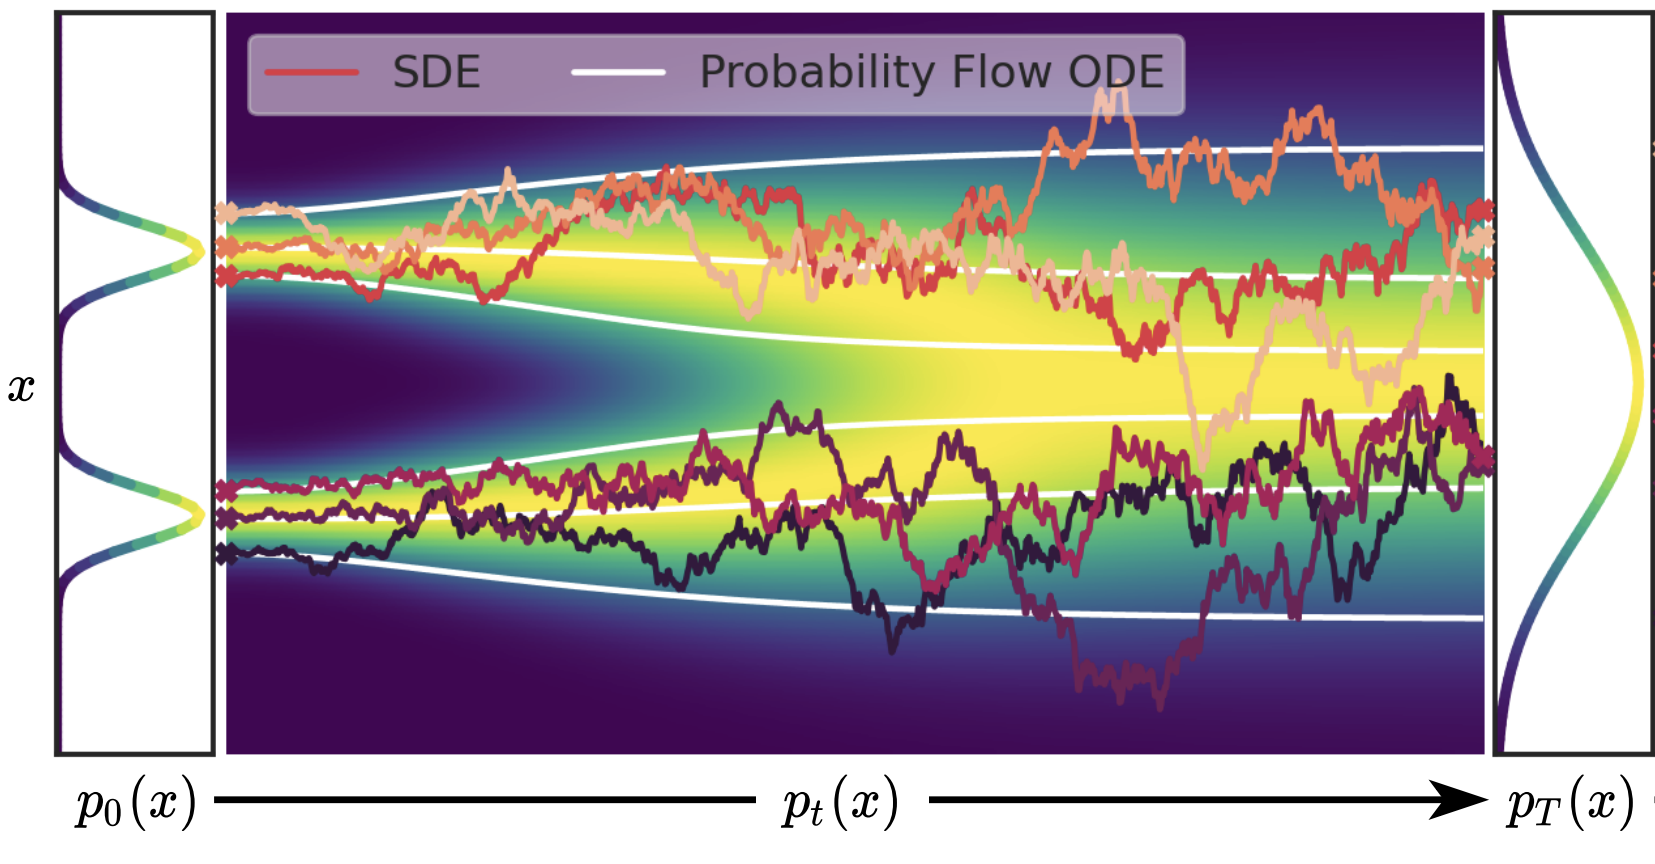
\includegraphics[width=0.75\linewidth]{figs/probability_flow}
	\end{figure}
\end{frame}
%=======
\begin{frame}{Recap of Previous Lecture}
	\myfootnotewithlink{https://arxiv.org/abs/2011.13456}{Song Y., et al. Score-Based Generative Modeling through Stochastic Differential Equations, 2020}
	\[
		d\bx = \bv(\bx, t) dt, \quad \bx(t + dt) = \bx(t) + \bv(\bx, t) dt
	\]
	\vspace{-0.7cm}
	\begin{block}{Reverse ODE}
		Let $\tau = 1 - t$ ($d\tau = -dt$):
		\vspace{-0.3cm}
		\[
			d\bx = - \bv(\bx, 1 - \tau) d \tau
		\]
	\end{block}
	\vspace{-0.5cm}
	\begin{block}{Reverse SDE}
		There's a reverse SDE for $d\bx = \bff(\bx, t) dt + g(t) d\bw$ in the following form:
		\vspace{-0.3cm}
		\[
			d\bx = \left(\bff(\bx, t) {\color{violet}- g^2(t) \frac{\partial}{\partial \bx}\log p_t(\bx)}\right) dt + g(t) d \bar{\bw}, \quad dt < 0
		\]
	\end{block}
	\vspace{-0.5cm}
	\begin{block}{Sketch of the Proof}
		\begin{itemize}
			\item Convert the initial SDE to the probability flow ODE.
			\item Reverse the probability flow ODE.
			\item Convert the reverse probability flow ODE to the reverse SDE.
		\end{itemize}
	\end{block}
\end{frame}
%=======
\begin{frame}{Recap of Previous Lecture}
	\myfootnotewithlink{https://arxiv.org/abs/2011.13456}{Song Y., et al. Score-Based Generative Modeling through Stochastic Differential Equations, 2020}
	\[
		d\bx = \bff(\bx, t) dt + g(t) d \bw
	\]
	\vspace{-0.3cm}
	\[
		\bv(\bx, t) = \bff(\bx, t) - \frac{1}{2} g^2(t) \bs(\bx, t), \quad \text{where} \quad \bs(\bx, t) = \nabla_{\bx} \log p_t(\bx)
	\]
	\vspace{-0.5cm}
	\begin{align*}
		d\bx &= \bv(\bx, t) dt \;\; - \textbf{Probability Flow ODE} \\
		d\bx &= \bigl({\color{violet}\bv(\bx, t) - \frac{1}{2} g^2(t) \bs(\bx, t)}\bigr) dt + g(t) d \bar{\bw} \;\; - \textbf{Reverse SDE}
	\end{align*}
	\vspace{-0.7cm}
	\begin{figure}
		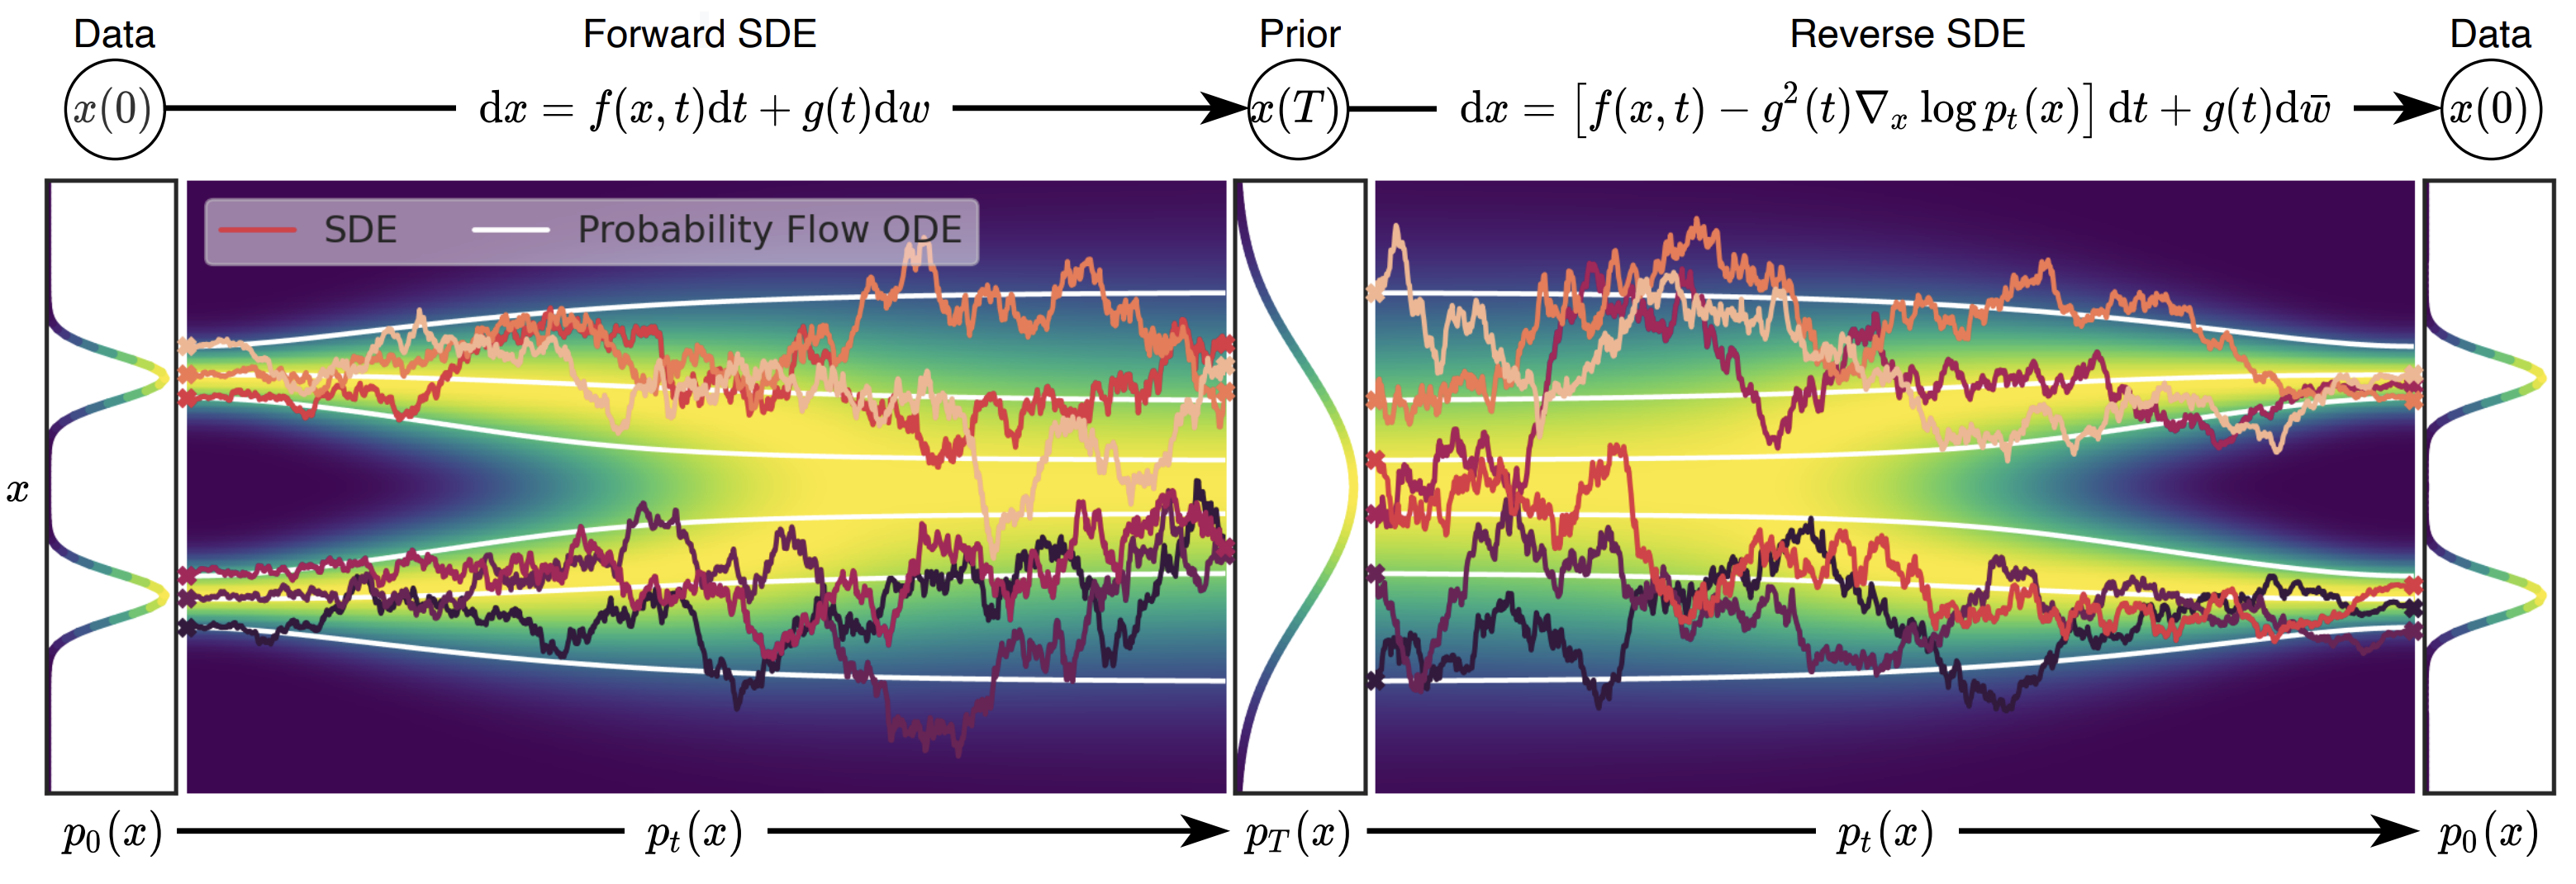
\includegraphics[width=1.0\linewidth]{figs/sde}
	\end{figure}
\end{frame}
%=======
\begin{frame}{Recap of Previous Lecture}
	\myfootnotewithlink{https://arxiv.org/abs/2011.13456}{Song Y., et al. Score-Based Generative Modeling through Stochastic Differential Equations, 2020}
	\begin{block}{Discrete-Time Objective}
		\vspace{-0.3cm}
		\[
			\bbE_{\pd(\bx_0)} \bbE_{t \sim U\{1, T\}} \bbE_{q(\bx_t | \bx_0)}\bigl\| \bs_{\btheta, t}(\bx_t) - \nabla_{\bx_t} \log q(\bx_t | \bx_0) \bigr\|^2_2 
		\]
		\vspace{-0.5cm}
	\end{block}
	\begin{block}{Continuous-Time Objective}
		\vspace{-0.5cm}
		\[
			\bbE_{\pd(\bx(0))} \bbE_{t \sim U[0, 1]} \bbE_{q(\bx(t) | \bx(0))}\bigl\| \bs_{\btheta}(\bx(t), t) - {\color{teal}\nabla_{\bx(t)} \log q(\bx(t) | \bx(0))} \bigr\|^2_2 
		\]
		\vspace{-0.5cm}
	\end{block}
	\begin{block}{NCSN}
		\vspace{-0.3cm}
		\[
			q(\bx(t) | \bx(0)) = \cN\left(\bx(0), \left[\sigma^2(t) - \sigma^2(0)\right] \cdot \bI\right)
		\]
		\vspace{-0.5cm}
	\end{block}
	\begin{block}{DDPM}
		\vspace{-0.5cm}
		\[
			q(\bx(t) | \bx(0)) = \cN\left(\bx(0) e^{-\frac{1}{2} \int_0^t\beta(s)ds}, \left(1 - e^{- \int_0^t\beta(s)ds}\right) \cdot \bI\right)
		\]
	\end{block}
	
\end{frame}
%=======
\begin{frame}{Recap of Previous Lecture}
	\myfootnotewithlink{https://arxiv.org/abs/2011.13456}{Song Y., et al. Score-Based Generative Modeling through Stochastic Differential Equations, 2020}
	\begin{block}{Sampling}
		To sample, solve the reverse SDE using numerical solvers (\SDESolve).
		\vspace{-0.3cm}
		\begin{figure}
			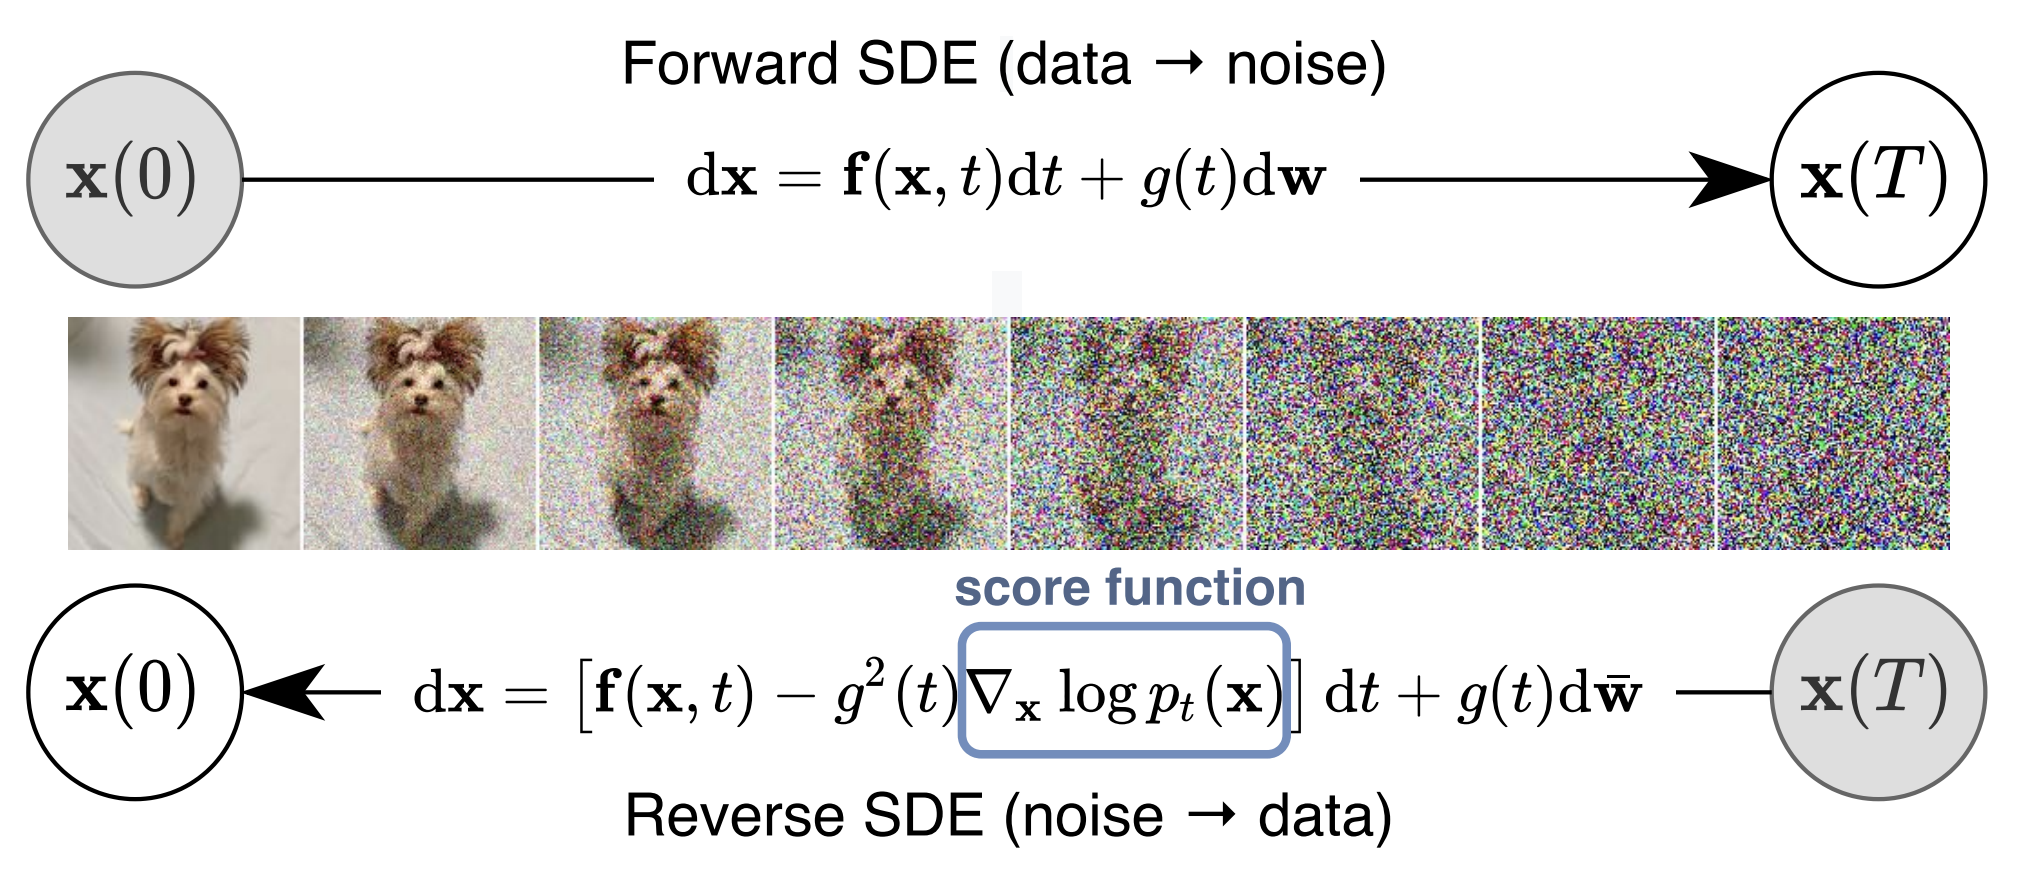
\includegraphics[width=0.8\linewidth]{figs/sbgm}
		\end{figure}
		\vspace{-0.5cm}
	\end{block}
	\begin{itemize}
		\item Discretizing the reverse SDE gives us ancestral sampling.
		\item If we use the probability flow ODE instead, then the reverse ODE yields DDIM sampling.
	\end{itemize}
\end{frame}
%=======
\begin{frame}{Recap of Previous Lecture}
	\myfootnotewithlink{https://arxiv.org/abs/2210.02747}{Lipman Y., et al. Flow Matching for Generative Modeling, 2022}
	Consider ODE dynamics $\bx(t)$ in the interval $t \in [0, 1]$ with $\bx_0 \sim p_0(\bx) = \cN(0, \bI)$, $\bx_1 \sim p_1(\bx) =  \pd(\bx)$.
	\[
		\frac{d \bx}{dt} = \bv (\bx, t),  \quad \text{with initial condition $\bx(0) = \bx_0$}.
	\]
	\vspace{-0.5cm}
	\begin{block}{KFP Theorem (Continuity Equation)}
		\vspace{-0.5cm}
		\[
			\frac{\partial p_t(\bx)}{\partial t} = - \diver\left(\bv(\bx, t) p_t(\bx)\right) \Leftrightarrow \frac{d \log p_t(\bx(t))}{d t} = - \tr \left( \frac{\partial \bv(\bx(t), t)}{\partial \bx(t)} \right)
		\]
		\vspace{-0.5cm}
	\end{block}
	Solving the continuity equation ODE numerically is complicated and unstable.
	\begin{block}{Flow Matching}
		\vspace{-0.3cm}
		\[
			\bbE_{t \sim U[0, 1]} \bbE_{\bx \sim p_t(\bx)}\left\| \bv(\bx, t) - \bv_{\btheta}(\bx, t) \right\|^2 \rightarrow \min_{\btheta}
		\]
		\vspace{-0.3cm}
		Flow matching is a scalable approach to Neural ODEs.
	\end{block}
\end{frame}
%=======
\begin{frame}{Outline}
	\tableofcontents
\end{frame}
%=======
\section{Conditional Flow Matching (CFM)}
%=======
\begin{frame}{Generative Models Taxonomy}
	\renderTaxonomy{fm}
\end{frame}
%=======
\subsection{CFM Objective}
%=======
\begin{frame}{Flow Matching}
    \myfootnotewithlink{https://arxiv.org/abs/2302.00482}{Tong A., et al. Improving and Generalizing Flow-Based Generative Models with Minibatch Optimal Transport, 2023}
	Let's introduce the latent variable $\bz$:
	\[
		p_t(\bx) = \int p_t(\bx | \bz) p(\bz) d \bz 
	\]
	Here, $p_t(\bx | \bz)$ is a \textbf{conditional probability path}.
	\eqpause
	The conditional probability path $p_t(\bx | \bz)$ satisfies the KFP theorem:
	\[
		\frac{\partial p_t(\bx | \bz)}{\partial t} = - \diver\left(\bv(\bx, \bz, t) p_t(\bx | \bz)\right),
	\]
	where $\bv(\bx, \bz, t)$ is a \textbf{conditional vector field}:
	\eqpause
	\[
		\frac{d\bx_t}{dt} = \bv(\bx_t, t) \quad \Rightarrow \quad \frac{d\bx_t}{dt} = \bv(\bx_t, \bz, t)
	\]
	\vspace{-0.3cm}
\end{frame}
%=======
\begin{frame}{Conditional Vector Field}
    \myfootnotewithlink{https://arxiv.org/abs/2302.00482}{Tong A., et al. Improving and Generalizing Flow-Based Generative Models with Minibatch Optimal Transport, 2023}
	\[
		{\color{violet}\frac{\partial p_t(\bx | \bz)}{\partial t} = - \diver\left(\bv(\bx, \bz, t) p_t(\bx | \bz)\right)},
	\]

	What's the relationship between $\bv(\bx, t)$ and $\bv(\bx, \bz, t)$?
	\eqpause
	\begin{block}{Theorem}
		The following vector field generates the probability path $p_t(\bx)$:
		\vspace{-0.3cm}
		\[
			\bv(\bx, t) = \bbE_{p_t(\bz | \bx)} \bv(\bx, \bz, t)  = {\color{teal}\int \bv(\bx, \bz, t)} \frac{\color{teal}p_t(\bx | \bz) p(\bz)}{p_t(\bx)} {\color{teal}d \bz}
		\]
		\vspace{-0.7cm}
	\end{block}
    \eqpause
	\begin{block}{Proof}
		\vspace{-0.7cm}
		\begin{multline*}
			\frac{\partial p_t(\bx)}{\partial t} = \frac{\partial}{\partial t} \int p_t(\bx | \bz) p(\bz) d \bz 
			\nextonslide{=  \int \left( {\color{violet} \frac{\partial p_t(\bx | \bz)}{\partial t} } \right) p(\bz) d \bz}
			\nextonslide{ = \\ = \int \left( {\color{violet} - \diver\left(\bv(\bx, \bz, t) p_t(\bx | \bz)\right) } \right) p(\bz) d \bz}
			\nextonslide{ = \\ = - \diver \left({\color{teal}\int \bv(\bx, \bz, t) p_t(\bx | \bz) p(\bz) d \bz }\right)} 
			\nextonslide{= - \diver  \left(\bv(\bx, t) p_t(\bx)\right)}
		\end{multline*}
	\end{block}
\end{frame}
%=======
\begin{frame}{Flow Matching}
    \myfootnotewithlink{https://arxiv.org/abs/2302.00482}{Tong A., et al. Improving and Generalizing Flow-Based Generative Models with Minibatch Optimal Transport, 2023}
	\begin{block}{Flow Matching (FM)}
		\vspace{-0.3cm}
		\[
			\bbE_{t \sim U[0, 1]} \bbE_{\bx \sim p_t(\bx)}\left\| \bv(\bx, t) - \bv_{\btheta}(\bx, t) \right\|^2 \rightarrow \min_{\btheta}
		\]
		\vspace{-0.3cm}
	\end{block}
	\begin{block}{Conditional Flow Matching (CFM)}
		\vspace{-0.3cm}
		\[
			\bbE_{t \sim U[0, 1]} \bbE_{\bz \sim p(\bz)} \bbE_{\bx \sim p_t(\bx | \bz)}\left\| \bv(\bx, \bz, t) - \bv_{\btheta}(\bx, t) \right\|^2 \rightarrow \min_{\btheta}
		\]
		\vspace{-0.5cm}
	\end{block}
    \eqpause
	\begin{block}{Theorem}
		If $\supp(p_t(\bx)) = \bbR^m$, then the optimal value of the FM objective equals the optimal value of the CFM objective.
	\end{block}
    \eqpause
	\begin{block}{Proof}
		This can be proved in a similar way as in the denoising score matching theorem.
	\end{block}
\end{frame}
%=======
\begin{frame}{Conditional Flow Matching}
    \myfootnotewithlink{https://arxiv.org/abs/2302.00482}{Tong A., et al. Improving and Generalizing Flow-Based Generative Models with Minibatch Optimal Transport, 2023}
	\begin{block}{Theorem}
		\vspace{-0.7cm}
		\begin{multline*}
			\argmin_{\btheta} \bbE_{t \sim U[0, 1]} \bbE_{\bx \sim p_t(\bx)}\left\| \bv(\bx, t) - \bv_{\btheta}(\bx, t) \right\|^2 = \\
			= \argmin_{\btheta} \bbE_{t \sim U[0, 1]} \bbE_{\bz \sim p(\bz)} \bbE_{\bx \sim p_t(\bx | \bz)}\left\| \bv(\bx, \bz, t) - \bv_{\btheta}(\bx, t) \right\|^2
		\end{multline*}
		\vspace{-0.7cm}
	\end{block}
    \eqpause
	\begin{block}{Proof}
		\vspace{-0.5cm}
		{\small
		\begin{multline*}
			\bbE_{\bx \sim p_t(\bx)}\left\| \bv(\bx, t) - \bv_{\btheta}(\bx, t) \right\|^2 = \\ 
			= {\color{olive}\bbE_{\bz \sim p(\bz)} \bbE_{\bx \sim p_t(\bx | \bz)}}\left[\| \bv_{\btheta}(\bx, t) \|^2 - 2 {\color{teal}\bv_{\btheta}^\top(\bx, t)\bv(\bx, t)} \right] + \text{const}(\btheta)
		\end{multline*}
		}
		\eqpause
		\vspace{-1.0cm}
		{\small
		\begin{multline*}
			\bbE_{p_t(\bx)} \left[{\color{teal}\bv_{\btheta}^\top(\bx, t)\bv(\bx, t)} \right] = \int p_t(\bx) \left[\bv_{\btheta}^\top(\bx, t) \left( \int p_t(\bz | \bx)\bv(\bx, \bz, t)d\bz \right) \right] d\bx 
			\nextonslide{ = \\ = \int \int {\color{violet}p_t(\bx) p_t(\bz | \bx)} \left[\bv_{\btheta}^\top(\bx, t) \bv(\bx, \bz, t) \right] d\bz d\bx}
			\nextonslide{ = \\ = {\color{violet}\bbE_{p(\bz)} \bbE_{p_t(\bx | \bz)}} \left[\bv_{\btheta}^\top(\bx, t) \bv(\bx, \bz, t) \right]}
		\end{multline*}
		}
	\end{block}
\end{frame}
%=======
\begin{frame}{Conditional Flow Matching: Training and Sampling}
	\myfootnotewithlink{https://arxiv.org/abs/2210.02747}{Lipman Y., et al. Flow Matching for Generative Modeling, 2022}
	\[
		\bbE_{t \sim U[0, 1]} \bbE_{\bz \sim p(\bz)} \bbE_{\bx \sim p_t(\bx | \bz)}\left\| \bv(\bx, \bz, t) - \bv_{\btheta}(\bx, t) \right\|^2 \rightarrow \min_{\btheta}
	\]
	\[
		\bbE_{p(\bz)} p_0(\bx | \bz) = \cN(0, \bI); \quad \bbE_{p(\bz)} p_1(\bx | \bz) = \pd(\bx).
	\]
	\eqpause
	\vspace{-0.3cm}
	\begin{block}{Training}
		\begin{enumerate}
			\item Sample $t \sim U[0, 1]$, $\bz \sim p(\bz)$, $\bx_t \sim p_t(\bx | \bz)$.
			\item Compute loss $ \cL = \left\| \bv(\bx_t, \bz, t) - \bv_{\btheta}(\bx_t, t) \right\|^2 $.
		\end{enumerate}
	\end{block}
	\eqpause
	\begin{block}{Sampling}
		\begin{enumerate}
			\item Sample $\bx_0 \sim \cN(0, \bI)$.
			\item Solve the ODE to obtain $\bx_1$:
			\vspace{-0.3cm}
			\[
				\bx_1 = \bpsi_1(\bx_0) = \ODESolve_v(\bx_0, \btheta, t_0=0, t_1=1).
			\]
		\end{enumerate}
	\end{block}
\end{frame}
%=======
\begin{frame}{Marginal-to-Conditional: Scores vs Velocities}
	\begin{block}{Denoising Score Matching}
		\vspace{-0.3cm}
		\[
			\bbE_{\pd(\bx)} \bbE_{q(\bx_{\sigma} | \bx)}\left\| \bs_{\btheta, \sigma}(\bx_{\sigma}) - \nabla_{\bx_{\sigma}} \log q(\bx_{\sigma} | \bx) \right\|_2^2 \rightarrow \min_{\btheta}
		\]
		\vspace{-0.3cm}
	\end{block}
	Optimal predictor: $\bs_{\btheta^*, \sigma}(\bx_\sigma) = \bbE_{q(\bx | \bx_\sigma)} \left[\nabla_{\bx_\sigma} \log q(\bx_\sigma | \bx) \right] = \nabla_{\bx_\sigma} \log q(\bx_\sigma)$
	\eqpause
	\begin{block}{Conditional Flow Matching}
		\vspace{-0.3cm}
		\[
			\bbE_{t \sim U[0, 1]} \bbE_{\bz \sim p(\bz)} \bbE_{\bx \sim p_t(\bx | \bz)}\left\| \bv(\bx, \bz, t) - \bv_{\btheta}(\bx, t) \right\|^2 \rightarrow \min_{\btheta}
		\]
		\vspace{-0.3cm}
	\end{block}
	Optimal predictor: $\bv_{\btheta^*}(\bx, t) = \bbE_{p_t(\bz | \bx)} \bv(\bx, \bz, t) = \bv(\bx, t)$. \\
	\eqpause
	\vspace{0.2cm}
	In both cases, the optimal MSE predictor is the posterior mean of the \textbf{conditional} target, which equals the intractable \textbf{marginal} quantity (score or velocity).
\end{frame}
%=======
\subsection{Conditional Probability Paths}
%=======
\begin{frame}{Conditional Flow Matching: Continuity Equations}
	\myfootnotewithlink{https://arxiv.org/abs/2510.21890}{Lai C. H. et al. The principles of diffusion models, 2025.}
	\begin{block}{Continuity Equations}
		\vspace{-0.5cm}
		\begin{align*}
			\frac{\partial p_t(\bx)}{\partial t} &= - \diver\left(\bv(\bx, t) \cdot p_t(\bx)\right) \\
			\frac{\partial p_t(\bx | \bz)}{\partial t} &= - \diver\left(\bv(\bx, \bz, t) \cdot p_t(\bx | \bz)\right)
		\end{align*}
		\vspace{-0.5cm}
	\end{block}
	What is the relationship between $p_t(\bx)$ and $\bv(\bx, t)$?
	\eqpause
	\begin{itemize}
		\item $\bv(\bx, t)$ (under regularity conditions) and initial condition $p_0(\bx)$ uniquely determine $p_t(\bx)$.
		\eqpause
		\item But the reverse is not true: any divergence-free vector field $\diver(\tilde{\bv}(\bx, t)p_t(\bx)) = 0$ can generate a valid probability path.
		\eqpause
		\item Moreover, not every given path $p_t(\bx)$ can actually arise from particles moving under
		some velocity field $\bv(\bx, t)$.
	\end{itemize}
\end{frame}
%=======
\begin{frame}{Conditional Flow Matching: Paths and Vector Fields}
	\begin{block}{Probability Paths}
		\vspace{-0.3cm}
		\[
			p_t(\bx) = \int p_t(\bx | \bz) p(\bz) d \bz
		\]
		\vspace{-0.5cm}
	\end{block}
	\eqpause
	\begin{itemize}
		\item $p_t(\bx | \bz)$ and $p(\bz)$ uniquely determine $p_t(\bx)$.
		\item The reverse is not true: many different conditional families integrate to the same marginal.
	\end{itemize}
	\eqpause
	\begin{block}{Vector fields}
		\vspace{-0.3cm}
		\[
			\bv(\bx, t) = \bbE_{p_t(\bz | \bx)} \bv(\bx, \bz, t) = \int \bv(\bx, \bz, t) \frac{p_t(\bx | \bz) p(\bz)}{p_t(\bx)} d \bz
		\]
		\vspace{-0.5cm}
	\end{block}
	\eqpause
	\begin{itemize}
		\item $\bv(\bx, \bz, t)$ and $p_t(\bx | \bz)$ uniquely determine $\bv(\bx, t)$.
		\item But marginal velocity does not determine conditional velocities (many decompositions exist).
	\end{itemize}
\end{frame}
%=======
\begin{frame}{From Marginal to Conditional Paths}
    \myfootnotewithlink{https://dl.heeere.com/conditional-flow-matching/blog/conditional-flow-matching}{image credit: A Visual Dive into Conditional Flow Matching}
	\begin{figure}
		\centering
		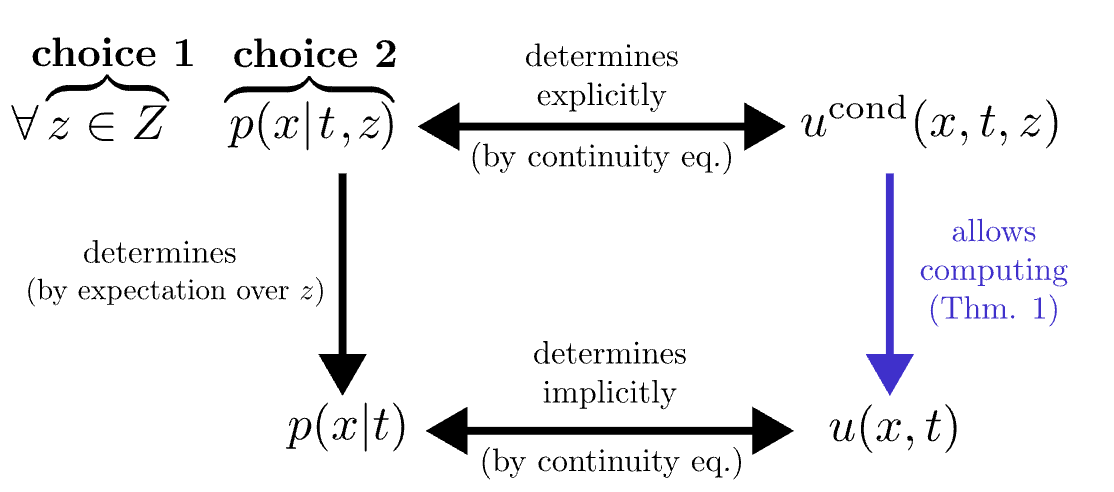
\includegraphics[width=0.75\linewidth]{figs/cfm_uncond_to_cond}
	\end{figure}
    \eqpause
	\begin{block}{Open Questions}
		\begin{itemize}
			\item[Q1] How should we choose the convenient conditioning latent variable $\bz$?
			\item[Q2] How can we parametrize $p_t(\bx)$ (or $p_t(\bx | \bz)$) to enforce the following constraints?
			\[
				\bbE_{p(\bz)} p_0(\bx | \bz) = \cN(0, \bI); \quad \bbE_{p(\bz)} p_1(\bx | \bz)= \pd(\bx).
			\]
		\end{itemize}
	\end{block}
\end{frame}
%=======
\begin{frame}{Gaussian Conditional Probability Paths [Q2]}
	\myfootnotewithlink{https://arxiv.org/abs/2302.00482}{Tong A., et al. Improving and Generalizing Flow-Based Generative Models with Minibatch Optimal Transport, 2023}
	Let's consider the following parametrization:
	\vspace{-0.3cm}
	\[
		p_t(\bx | \bz) = \cN\left(\bmu_t(\bz), \bsigma_t^2(\bz) \right)
	\]
	\eqpause
	The concrete $\bmu_t(\bz)$, $\bsigma_t(\bz)$ (which satisfy the boundary constraints) will be fixed once we choose $\bz$ [Q1].
	\begin{block}{Gaussian flow}
		\begin{itemize}
			\item Let's derive the vector field for \textbf{any} Gaussian path $p_t(\bx | \bz)$.
			\item There are infinitely many flows $\bpsi_t(\bx_0, \bz)$ (or, equivalently, vector fields $\bv(\bx_t, \bz, t)$) that generate a particular probability path $p_t(\bx | \bz)$.
			\eqpause
			\item Let's consider the following flow:
			\vspace{-0.3cm}
			\[
				\bx_t = \bpsi_t(\bx_0, \bz) = \bmu_t(\bz) + \bsigma_t(\bz) \odot \bepsilon,
			\]
			where $\bepsilon$ is fixed by the condition: $\bx_0 = \bmu_0(\bz) + \bsigma_0(\bz) \odot \bepsilon$.
		\end{itemize}
	\end{block}
\end{frame}
%=======
\begin{frame}{Gaussian Conditional Vector Field}
	\myfootnotewithlink{https://arxiv.org/abs/2302.00482}{Tong A., et al. Improving and Generalizing Flow-Based Generative Models with Minibatch Optimal Transport, 2023}
	\begin{block}{Gaussian Conditional Probability Path}
		\vspace{-0.5cm}
		\[
			p_t(\bx | \bz) = \cN\left(\bmu_t(\bz), \bsigma_t^2(\bz)\right); \quad \bx_t = \bpsi_t(\bx_0, \bz) = \bmu_t(\bz) + \bsigma_t(\bz) \odot \bepsilon
		\]
		\vspace{-0.5cm}
	\end{block}
	\eqpause
	How to derive the expression for $\bv(\bx_t, \bz, t)$ for this particular flow $\bpsi_t(\bx_0, \bz)$?
	\eqpause
	\vspace{-0.3cm}
	\[
		\frac{d\bx_t}{dt} = \bv(\bx_t, \bz, t); \quad {\color{violet}\bepsilon = \frac{1}{\bsigma_t(\bz)} \odot (\bx_t - \bmu_t(\bz))}
	\]
	\eqpause
	\[
		\frac{d\bx_t}{dt} = \bmu_t'(\bz) + \bsigma_t'(\bz) \odot {\color{violet}\bepsilon} 
	\]
	\eqpause
	\[
		\boxed{\bv(\bx_t, \bz, t) = \bpsi_t'\left(\bpsi_t(\bx_t, \bz)^{-1}, \bz\right) = \bmu_t'(\bz) + \frac{\bsigma_t'(\bz)}{\bsigma_t(\bz)} \odot (\bx_t - \bmu_t(\bz))}
	\]
\end{frame}
%=======
\section{One-Sided Conditioning}
%=======
\begin{frame}{Endpoint Conditioning}
	\myfootnotewithlink{https://arxiv.org/abs/2210.02747}{Lipman Y., et al. Flow Matching for Generative Modeling, 2022}
	\begin{block}{Conditional Flow Matching}
		\vspace{-0.5cm}
		\[
			\bbE_{t \sim U[0, 1]} \bbE_{\bz \sim p(\bz)} \bbE_{\bx \sim p_t(\bx | \bz)}\left\| \bv(\bx, \bz, t) - \bv_{\btheta}(\bx, t) \right\|^2 \rightarrow \min_{\btheta}
		\]
		\vspace{-0.5cm}
	\end{block}
	Let's define our latent variable $\bz$.
	\eqpause
	\begin{block}{Conditioning Latent Variable [Q1]}
		Let us choose $\bz = \bx_1$. Then $p(\bz) = p_1(\bx_1)$.
		\[
			p_t(\bx) = \int p_t(\bx | \bx_1) p_1(\bx_1) d \bx_1
		\]
	\end{block}
	\vspace{-0.3cm}
	\eqpause
	We need to ensure the boundary constraints:
	\[
		\begin{cases}
			\bbE_{p(\bz)} p_0(\bx | \bz) = \cN(0, \bI) \\
			\bbE_{p(\bz)} p_1(\bx | \bz) = \pd(\bx)
		\end{cases}
		\quad 
		\nextonslide{
			\Rightarrow \quad 
			\begin{cases}
				p_0(\bx | \bx_1) = \cN(0, \bI); \\
				p_1(\bx | \bx_1) = \delta(\bx - \bx_1)
			\end{cases}
		}
	\]
	\vspace{-0.3cm}
\end{frame}
%=======
\begin{frame}{One-Sided Conditioning}
	\myfootnotewithlink{https://dl.heeere.com/conditional-flow-matching/blog/conditional-flow-matching}{image credit: A Visual Dive into Conditional Flow Matching}
	\[
		p_0(\bx | \bx_1) = \cN(0, \bI); \quad p_1(\bx | \bx_1) = \delta(\bx - \bx_1)
	\]

	\begin{block}{Gaussian Conditional Probability Path}
		\vspace{-0.5cm}
		\[
			p_t(\bx | \bx_1) = \cN\left(\bmu_t(\bx_1), \bsigma_t^2(\bx_1)\right); \quad \bx_t = \bmu_t(\bx_1) +  \bsigma_t(\bx_1) \odot {\color{olive}\bepsilon}
		\]
		\vspace{-0.7cm}
	\end{block}
	\eqpause
	\begin{figure}
		\centering
		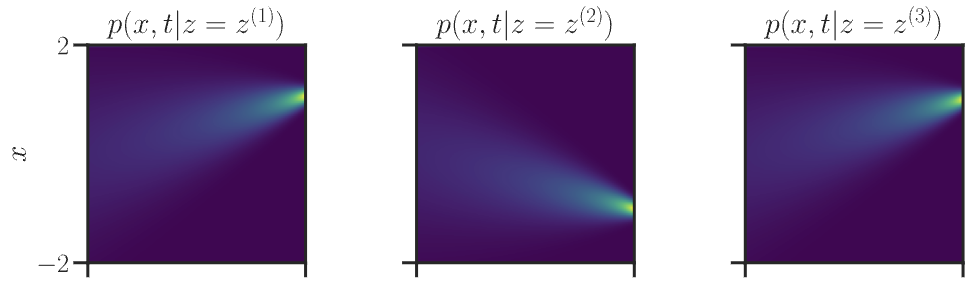
\includegraphics[width=\linewidth]{figs/conical_paths}
	\end{figure}
	\eqpause
	Let's consider straight conditional paths:	
	\[
		\begin{cases}
			\bmu_t(\bx_1) = t \bx_1 \\
			\bsigma_t(\bx_1) = 1 - t
		\end{cases}
		\quad 
		\nextonslide{
			\Rightarrow \quad 
			\begin{cases}
				p_t(\bx | \bx_1) = \cN\left(t \bx_1, (1-t)^2 \cdot \bI\right) \\
				\bx_t = t \bx_1 + (1 - t) {\color{olive}\bx_0}
			\end{cases}
		}
	\]
\end{frame}
%=======
\begin{frame}{One-Sided Conditioning: Conditional Vector Field}
	\myfootnotewithlink{https://mlg.eng.cam.ac.uk/blog/2024/01/20/flow-matching.html}{image credit: https://mlg.eng.cam.ac.uk/blog/2024/01/20/flow-matching.html}
	\[
		p_t(\bx | \bx_1) = \cN\left(t \bx_1, (1-t)^2 \bI\right); \quad {\color{teal}\bx_t = t \bx_1 + (1 - t) \bx_0}
	\]
	\vspace{-0.3cm}
	\begin{block}{Conditional Vector Field}
		\vspace{-0.3cm}
		\[
			 \frac{d\bx_t}{dt} = \bv(\bx_t, \bx_1, t) =  \bmu_t'(\bx_1) + \frac{\bsigma_t'(\bx_1)}{\bsigma_t(\bx_1)} \odot (\bx_t - \bmu_t(\bx_1))
		\]
		\eqpause
		\vspace{-0.5cm}
		\begin{multline*}
			\bv(\bx_t, \bx_1, t) = \bx_1 - \frac{1}{1-t} \cdot (\bx_t - t \bx_1) 
			= \frac{\bx_1 - {\color{teal}\bx_t}}{1-t}
			\nextonslide{ = \\ = \frac{\bx_1 - {\color{teal}t \bx_1 - (1 - t) \bx_0}}{1-t}}
			\nextonslide{= \bx_1 - \bx_0}
		\end{multline*}
	\end{block}
	\eqpause
	\vspace{-0.5cm}
	\begin{minipage}[t]{0.55\columnwidth}
		\vspace{-0.7cm}
		\begin{figure}
			\centering
			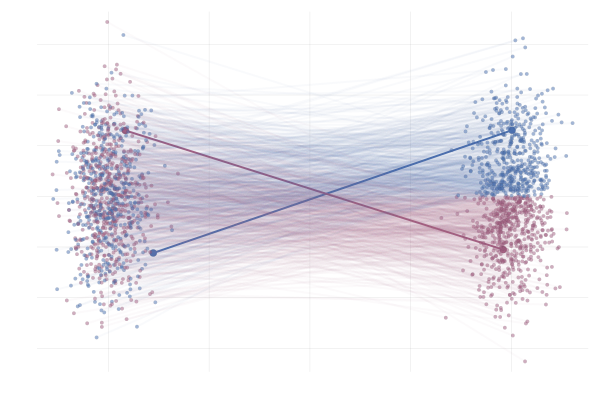
\includegraphics[width=0.9\linewidth]{figs/g2g-vector-field-samples-cond}
		\end{figure}
	\end{minipage}%
	\begin{minipage}[t]{0.45\columnwidth}
		The conditional vector field $\bv(\bx_t, \bx_1, t)$ defines straight lines between $\pd(\bx)$ and $\cN(0, \bI)$.
	\end{minipage}
\end{frame}
%=======
\begin{frame}{One-Sided Conditioning: CFM Objective}
	\myfootnotewithlink{https://arxiv.org/abs/2210.02747}{Lipman Y., et al. Flow Matching for Generative Modeling, 2022}
	\vspace{-0.5cm}
	\begin{multline*}
		\bbE_{t \sim U[0, 1]} \bbE_{\bz \sim p(\bz)} \bbE_{\bx \sim p_t(\bx | \bz)}\left\| {\color{olive}\bv(\bx, \bz, t)} - \bv_{\btheta}(\bx, t) \right\|^2
		= \\ = \bbE_{t \sim U[0, 1]} \bbE_{\bx_1 \sim \pd(\bx)} {\color{violet}\bbE_{\bx \sim p_t(\bx | \bx_1)}}\left\| {\color{olive}\frac{\bx_1 - \bx}{1-t}} - \bv_{\btheta}({\color{teal}\bx}, t) \right\|^2
		\nextonslide{ = \\ = \bbE_{t \sim U[0, 1]} \bbE_{\bx_1 \sim \pd(\bx)} {\color{violet}\bbE_{\bx_0 \sim \cN(0, \bI)}}\left\| (\bx_1 - \bx_0) - \bv_{\btheta}\left({\color{teal}t \bx_1 + (1 - t) \bx_0}, t\right) \right\|^2}
	\end{multline*}
	\eqpause
	\vspace{-0.5cm}
	\begin{itemize}
		\item We fit straight lines between the noise distribution $p_0(\bx)$ and the data distribution $\pd(\bx)$.
		\item The \textbf{marginal} path $p_t(\bx)$ does not give straight lines.
	\end{itemize}
	\eqpause
	\vspace{-0.3cm}
	\begin{minipage}[t]{0.5\columnwidth}
			\begin{figure}
				\centering
				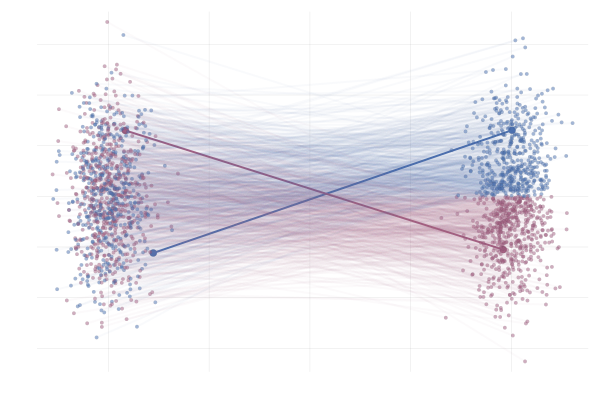
\includegraphics[width=\linewidth]{figs/g2g-vector-field-samples-cond}
			\end{figure}
		\end{minipage}%
		\begin{minipage}[t]{0.5\columnwidth}
			\begin{figure}
				\centering
				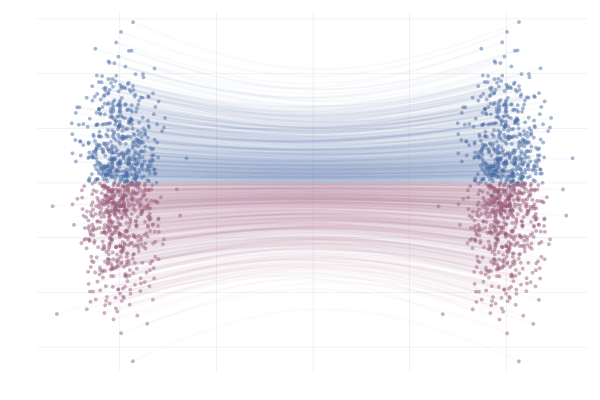
\includegraphics[width=\linewidth]{figs/g2g-forward_samples}
			\end{figure}
	\end{minipage}
\end{frame}
%=======
\begin{frame}{CFM with One-Sided Conditioning: Training and Sampling}
	\myfootnotewithlink{https://arxiv.org/abs/2210.02747}{Lipman Y., et al. Flow Matching for Generative Modeling, 2022}
	\vspace{-0.3cm}
	\[
	 \bbE_{t \sim U[0, 1]} \bbE_{\bx_1 \sim \pd(\bx)} \bbE_{\bx_0 \sim \cN(0, \bI)}\left\| (\bx_1 - \bx_0) - \bv_{\btheta}(\bx_t, t) \right\|^2  \rightarrow \min_{\btheta}
	\]
	\begin{block}{Training}
		\begin{enumerate}
			\item Sample $\bx_1 \sim \pd(\bx)$, $\bx_0 \sim \cN(0, \bI)$, $t \sim U[0, 1]$.
			\item Compute noisy image $\bx_t = t \bx_1 + (1 - t) \bx_0$.
			\item Compute loss $ \cL = \left\| (\bx_1 - \bx_0) - \bv_{\btheta}(\bx_t, t) \right\|^2 $.
		\end{enumerate}
	\end{block}
	\eqpause
	\vspace{-0.3cm}
	\begin{block}{Sampling}
		\begin{enumerate}
			\item Sample $\bx_0 \sim \cN(0, \bI)$.
			\item Solve the ODE to obtain $\bx_1$:
			\vspace{-0.3cm}
			\[
				\bx_1 = \bpsi_1(\bx_0) = \ODESolve_v(\bx_0, \btheta, t_0=0, t_1=1).
			\]
		\end{enumerate}
	\end{block}
\end{frame}
%=======
\begin{frame}{Conditional vs. Marginal Paths}
	\myfootnotewithlink{https://arxiv.org/abs/2506.02070}{Holderrieth P. and Erives E., et al. An Introduction to Flow Matching and Diffusion Models, 2025}
	\begin{figure}
		\centering
		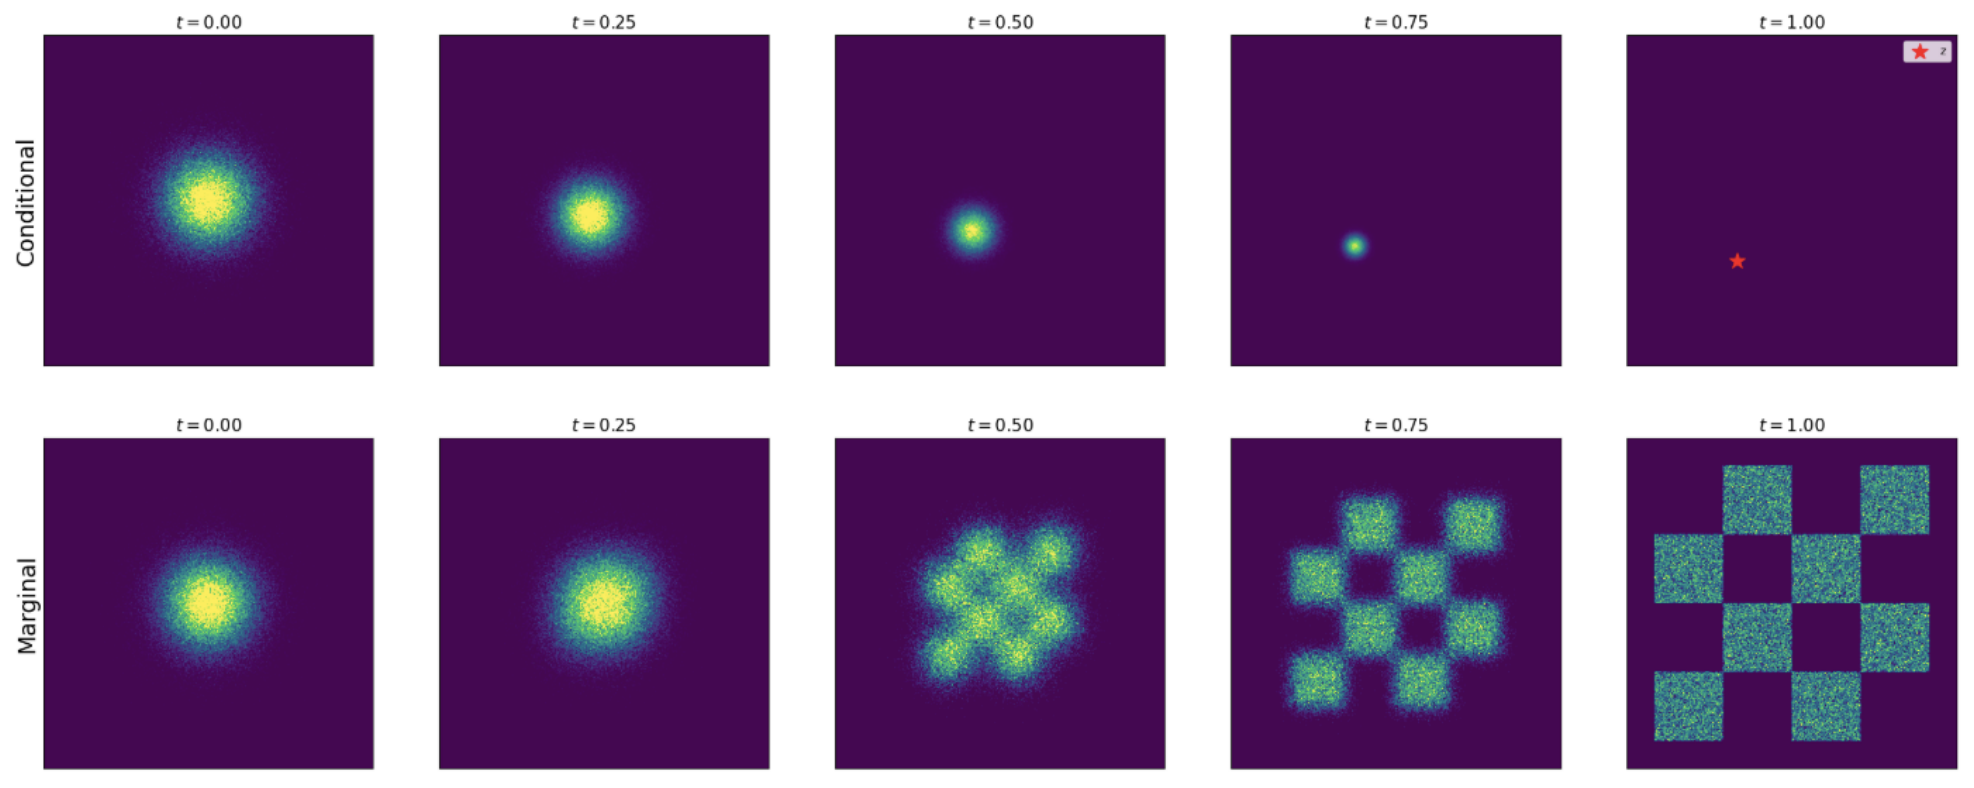
\includegraphics[width=\linewidth]{figs/cond_marg_paths}
	\end{figure}
	\eqpause
	\begin{itemize}
		\item One-sided conditioning gives us the way to construct a generative model.
		\item Now we extend it to image-to-image formulation (mapping between two distinct data distributions $p_0(\bx)$ and $p_1(\bx)$).
	\end{itemize}
\end{frame}
%=======
\begin{frame}{Summary}
	\begin{itemize}
		\item Conditional flow matching introduces the latent variable $\bz$, reformulating the initial task in terms of conditional dynamics.
		\vfill
		\item The marginal vector field can be expressed as the posterior mean of conditional vector fields: $\bv(\bx, t) = \bbE_{p_t(\bz | \bx)} \bv(\bx, \bz, t)$.
		\vfill
		\item The FM and CFM objectives have the same optimal solution, making CFM a tractable alternative to FM.
		\vfill
		\item For Gaussian conditional paths $p_t(\bx | \bz) = \cN(\bmu_t(\bz), \bsigma_t^2(\bz))$, the conditional vector field has a closed form for $\bv(\bx_t, \bz, t)$.
		\vfill
		\item One-sided conditioning uses endpoint conditioning $\bz = \bx_1$ with straight conditional paths, yielding the simple vector field $\bv(\bx_t, \bx_1, t) = \bx_1 - \bx_0$.
	\end{itemize}
\end{frame}
%=======
\end{document}